\chapter{MicroPython IDE} \label{ide}

\section{Connecting Your Microcontroller}
Throughout this guide, we will be making use of a free online IDE for connecting our microcontroller
to our computer and loading, editing, and running code on it. You can access the IDE from your browser
by going to \url{https://viper-ide.org/}. Click on the USB icon in the top right and choose your
microcontroller from the list:

\begin{figure}[H]
    \centering
    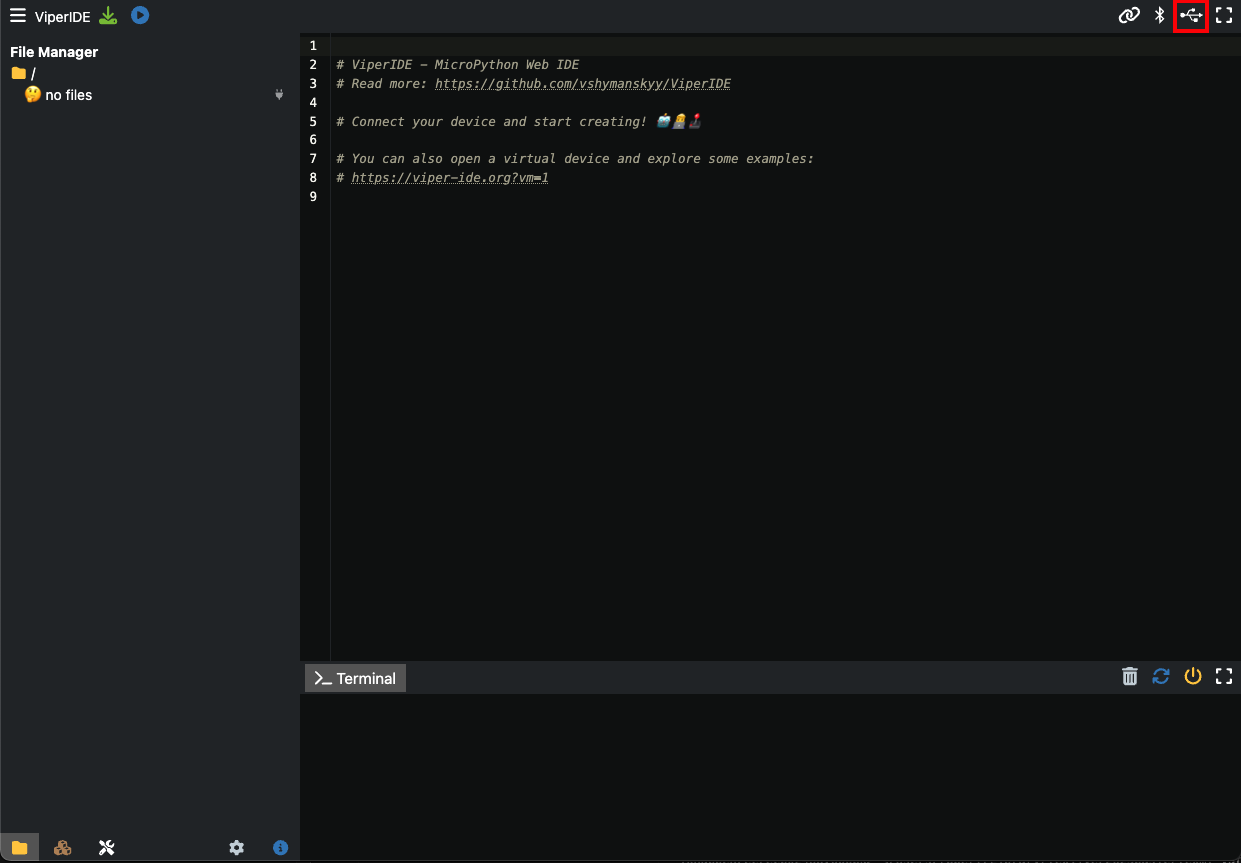
\includegraphics[width=.8\linewidth]{common/viper_ide_usb_connect.png}
    \caption{Click the button highlighted in red.}
\end{figure}

If you see multiple items in the dialog that pops up, choose the one that starts with "USB JTAG". See below for an example:
\begin{figure}[H]
    \centering
    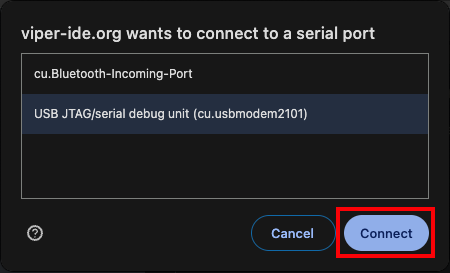
\includegraphics[width=.6\linewidth]{common/viper_ide_usb_choice_connect.png}
    \caption{Click the button highlighted in red.}
\end{figure}

Once you have connected, you will see a green dialog labeled "Device connected" and the file manager on the list
will populate with the list of files installed on the device:
\begin{figure}[H]
    \centering
    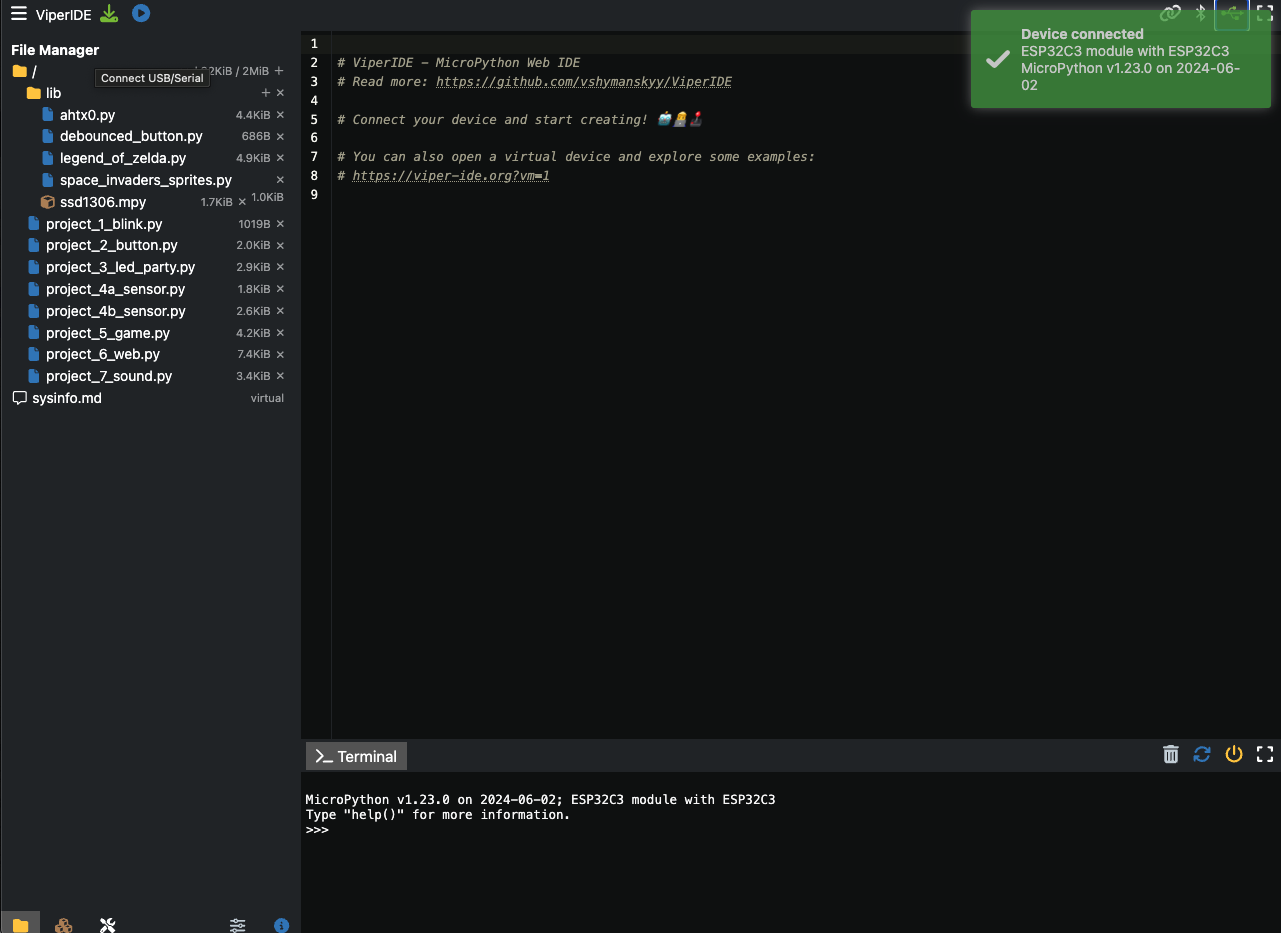
\includegraphics[width=\linewidth]{common/viper_connected.png}
    \caption{Make sure to open the right file for this project}
\end{figure}

After your device is connected, refer back to the chapter you are working on for the next steps.
